\subsection{Il medico condotto}

Al termine della scorsa lezione eravamo arrivati a parlare del concetto
di medico di Condotta. Questo concetto risale ad un'epoca alto
medievale, al passaggio al XIII secolo. C'erano già state delle
strutture presso l'impero e questo era stato un successo di Galeno
all'imperatore Marco Aurelio. Di fatto si parlava di strutture come
degli ambulatori pubblici in cui venivano curati i non abbienti.
Ovviamente erano presieduti da un medico e da una cerchia di figure con
funzioni di guaritori (es. Cerusici, Omatari,..). Il passaggio
conventuale, nell'Alto Medioevo, è stato fondamentale e si fondò sul
concetto della Pietas. Il concetto dell'ospizio era quello di offrire
alla popolazione povera un'alimentazione adeguata, quindi cibo
sufficiente, e ambienti sani e igienici. In realtà, secondo le
testimonianze del tempo, il mantenimento di norme igienico-sanitarie
adeguate non era sempre possibile e soprattutto nei momenti di crisi, si
potevano trovare all'interno di questi ambulatori, letti con più
pazienti contemporaneamente. Fra l'XI e il XIII secolo si arriva alla
definizione vera e propria di condotte, perché la chiesa comincia a
ritirarsi dagli impegni in ambito di salute. Vigeva la regola per cui il
Monaco non faceva tutto ma in alcuni casi intervenivano altre figure, i
medici letterates o chirurghi rurales, che erano quelli che si
prendevano cura delle popolazioni al di fuori delle città murarie.
\\\\
Quindi perché condotta? Viene dal termine condurre, che ha in sé la
stessa radice di condottiero. Il condottiero è una figura, che veniva
pagata per mestiere per fare la guerra e durante la guerra era a capo di
un gruppo di soldati. Allo stesso modo il condotto è la figura, in
ambito della salute, che veniva pagata per fare determinate cose. Questi
condotti stipulavano dei contratti di guarigione, sia con le strutture
comunali, ecclesiastiche, ma anche con i pazienti stessi, attraverso cui
venivano pagati. Il concetto di valutazione dell'operato sanitario di un
professionista in un certo modo nasce in questo momento.
\\\\
Per fare un esempio riporto un contratto di Guarigione stipulato fra un
medico e un paziente. Nel contratto viene specificata qual è l'infermità
del paziente ``nella mano nel piede e in bocca''. Viene anche indicato
un termine di misurazione dell'efficacia dell'intervento sanitario,
``entro 1 mese e mezzo''. Dobbiamo pensare al concetto moderno di
valutazione della qualità, in cui vengono costituiti dei criteri, in
base ai quali giudicare se si è ottenuto o meno un risultato; qui è già
presente. Nella lettera viene fatto l'esempio di ``tagliare il pane e
calzarti e camminare e parlare'' per riferire come il paziente guarirà
dal problema riferito al piede, alla mano e alla bocca. Il medico per
poter portare a termine la guarigione del paziente necessita, come
specificato, di poter fare tutte le spese che gli sono necessarie, e
quindi di essere pagato (7 Lire genovesi). Viene quindi stabilito il
sistema di remunerazione e il medico promette di non farsi pagare,
qualora l'intervento sanitario non sia efficace (``Se non manterrò con
te queste promesse non mi devi dare niente''). Si può notare inoltre la
terapia, che il paziente deve seguire, che seguiva le idee del tempo (né
frutta, né carne di bue, né pasta bollita o asciutta, né cavoli).

\begin{figure}[!ht]
\centering
	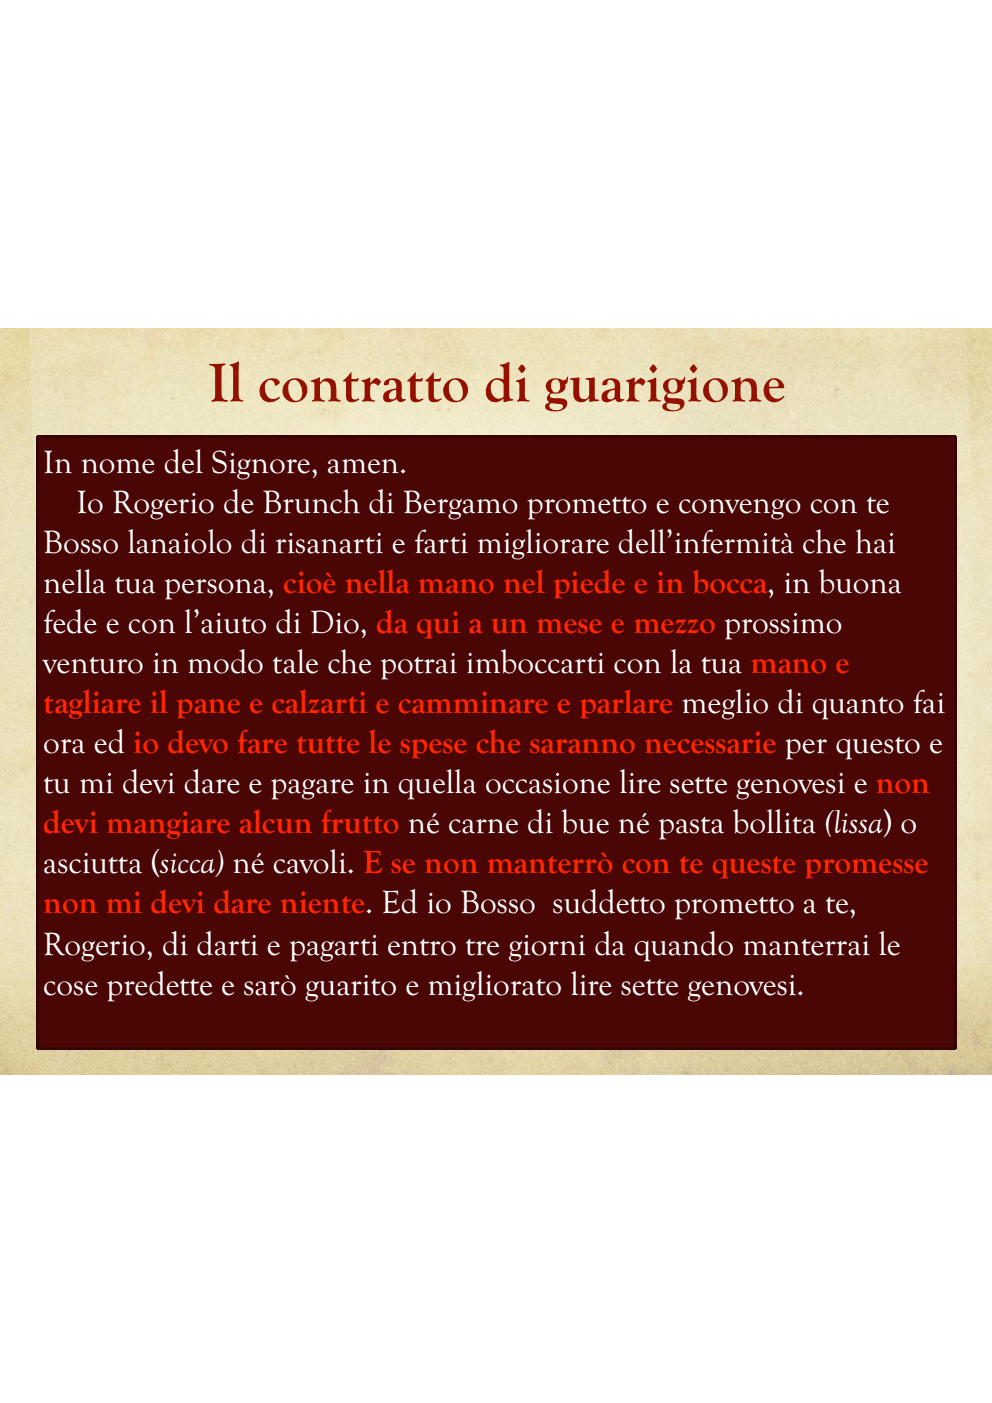
\includegraphics[width=0.8\textwidth]{38/image1.png}
	\end{figure}

Il primo stato, che codificò il sistema delle condotte, fu il Piemonte
con una legge del 1711. Con la definizione di Condotta piena, che verrà
eliminata solo nel 1923, si intendeva l'assistenza gratuita alla
popolazione povera. Il tempo è pieno, non ci sono limiti di orario, per
tutto l'anno e lo stipendio è basso. Non sono previsti in alcun caso,
nei contratti del 1700, delle prestazioni a pagamento esterno. Non era
previsto pensionamento. In caso di malattia, il medico doveva trovare un
sostituto a pagamento. Anche se in Piemonte la condotta si stabilisce
presto, non ha grande diffusione (es. la Valle d'Aosta non ne possiede,
la Val di Susa ne possiede poche). Diversa la situazione nel Lombardo-
Veneto, dove la condotta medica raggiunse risultati numericamente e
qualitativamente tra i più rilevanti.
\\\\
La regina d'Austria Maria Teresa propose una riforma Sanitaria molto
importante. Questa riforma è così avanzata che ha addirittura interesse
per la vaccinazione, contro il Vaiolo. Considera importanti i problemi
della salute e i mezzi con cui prevenire e controllarle. In questa
riforma si inquadra la costituzione in Lombardia del Direttorio medico,
il cui responsabile nel 1870 fu il Professore Johann Peter Frank.
\\\\
Frank ottenne anche una cattedra in medicina interna e pratica
all'università di Pavia e qui sconvolse completamente l'insegnamento di
medicina. Rese talmente rinomata l'Università da superare il confronto
con il numero di iscrizioni che annualmente si registravano
all'università di Legge (Nel 1793 gli iscritti a medicina sono 107 a
fronte di 800 iscritti alla Facoltà di legge; Nel 1796 ci sono 1000
iscritti a medicina e un centinaio iscritti a legge. Questi numeri fanno
capire il cambiamento).

Frank fece un'analisi di qual era l 'assistenza prevista nei vari
distretti di Milano, sia qualitativamente che quantitativamente, e
riorganizzò il sistema. Dall'analisi emerse una distribuzione ineguale
delle condotte che venne attribuita a:

\begin{itemize}
\item
  alla scarsa e incerta remunerazione dei condotti;
\item
  alla loro condizione di subalternità ai rappresentati dei comuni, con
  la relativa precarietà del posto a seconda degli interessi in gioco;
\end{itemize}

Nominato responsabile del direttorio, Frank dettò le sue ``proposizioni
preliminari al piano della sistemazione medica della Lombardia
austriaca'', che delineavano il sistema delle condotte come una
responsabilità dello stato.

Frank inoltre introdusse l'obbligo per i condotti di inviare alla
Facoltà medica dei rapporti semestrali sulle malattie curate con
l'indicazione dei dati anagrafici dei pazienti, sul decorso clinico,
delle terapie usate e di considerazioni sulla natura dell'infermità,
entro quadri nosostatici preparati dagli stessi vertici delle
professioni sanitarie dello stato di Milano. Le facoltà di medicina
avevano un compito di controllo.
\\\\
Questa riforma non fu però ben accolta, i medici sono sempre un po'
lenti a recepire i cambiamenti. Medici ostili, notabili di campagna,
amministratori ospedalieri videro la riforma come ``arbitraria
dittatura''.

Nel 1795, all'arrivo dei francesi e di Napoleone, Frank fu richiamato a
Vienna e la riforma era ancora in gran parte sulla carta.
L'organizzazione della riforma era tale per cui fu mantenuta all'interno
del Regolamento Napoleonico.
\\\\
Il Regolamento napoleonico di polizia medica, emanato il 5 Settembre
1806, attribuiva il potere di attuarne i provvedimenti al Ministero
dell'interno del Regno d'Italia Napoleonico che tra l'altro doveva
assicurare una capillare distribuzione delle condotte mediche e
chirurgiche. Affidava alle facoltà di Medicina delle università di
Pavia, Padova e Bologna le funzioni di Direzioni mediche, con compiti di
vigilanza sul modo di operare delle condotte stesse.
\\\\
Dopo la restaurazione viene ripresa il concetto della ristrutturazione
delle condotte secondo quanto previsto da Frank e di fatto avviene anche
l'introduzione reale della vaccinazione contro il vaiolo. Questo
rappresenta il primo esempio strutturato di vaccinazione sistematica
della popolazione. L'obbligo di vaccinare viene affidata al medico
condotto. Ci sono alcuni comuni che introducono la condotta piene non
più solo per i più poveri ma anche per gli ``estimati'', quelli che
venivano censiti perché possedevano delle proprietà immobiliari.
Pressati così, i medici di condotta non avevano una vita facile. Il
lavoro era descritto come poco remunerato. In caso di malattia dovevano
ancora pagarsi il sostituto e inoltre dovevano possedere un cavallo per
potersi spostare.
\\\\
Nel 1861 nasce il Regno d'Italia, sotto la guida di Vittorio Emanuele II
di Savoia. Nella media gli analfabeti erano il 75\%, con punte del
85-90\% al Sud e nelle Isole, rispetto al 54\% del Nord. Arrivati
all'unità d'Italia chiaramente ci si trova di fronte ad una miriade di
legislazioni differenti. Proprio per questo motivo il 20 Marzo del 1865
esce un Decreto che riorganizza tutta la legislazione e anche la Sanità
Pubblica. Il ministero dell'Interno aveva le funzioni di tutela della
salute pubblica; la catena di responsabilità passava ai prefetti, ai
sottoprefetti e ai sindaci. Il ministero era coadiuvato da un consiglio
superiore di Sanità, i prefetti da consigli sanitari provinciali e
circondariali.
\\\\
Il primo spostamento consistente verso i bisogni reali del paese viene
fatto grazie a Agostino Bertani, medico, radicale appartenente alla
sinistra storica, e Agostino Depretis, ministro degli Interni. Va
ricordato che fino al 1950 non si parlerà mai di Ministero della Sanità,
i compiti in materia di Sanità sono affidati al Ministero degli Interni.
Bertani propone a tutti i medici d'Italia un questionario per sapere
quali fossero le condizioni esistenti in giro per il paese (
``questionario De pretis''). Dai risultati pubblicati nel 1886 emerse
che:

\begin{itemize}
\item
6404 Comuni in Italia non possiedono Fognature, questo fa capire quali
fossero le condizioni igienico sanitarie;
\item 1286 non possiedono latrine;
\item 1350 le immondezze si raccoglievano nei cortili;
\item 1142 non si provvedeva alla nettezza nelle vie, non c'era sistemi di
scolo nelle strade..
\end{itemize}

Le condotte tuttavia vengono rafforzate. Nel 1882 la media nazionale
faceva registrare il 93\% di comuni associati, in esclusiva o in
consorzio, ad un medico. I valori più bassi, paradossalmente si
registrarono in Piemonte (\textless{} 80\%). Nel Lombardo -veneto, forti
dell'amministrazione asburgica, nel 98\% del paese avevano una condotta.

Tuttavia permanevano gravi problemi di arretratezza. La popolazione
presentava ancora al tempo un'aspettativa di vita di soli 34,5 anni. Il
tasso di analfabetismo era del 62\% nel 1881, migliorato rispetto ai
primi dati dopo l'unità d' Italia (75\% media nazionale nel 1861).
\\\\
Legge Crispi-Pagliani (1888): Si istituisce la direzione sanitaria
presso il Ministero dell'Interno con l'assegnazione del relativo
responsabile. A dirigere l'ufficio viene chiamato Pagliani, professore
di Igiene all'Università di Torino e senatore. Cripsi, con la
collaborazione di Pagliani, predispone quindi un testo di riforma che,
in buona parte recependo i principi e le proposte di Bertani se ne
discostava per la snellezza del testo, contenuto in circa 70 articoli a
fronte dei 188 del codice Bertani.
\\\\
Con la legge viene stabilito che possono entrare nel governo della
sanità, per la prima volta, dei medici nei consigli provinciali. La
catena di gerarchia funzionale tecnico-sanitaria è ora Ministero degli
Interni, prefetto, viceprefetto, presidente della provincia; E in
ciascuna di queste strutture, istituto superiore di Sanità e consiglio
provinciale, c'erano inserite delle figure mediche. Si era così avviato
il ``governo'' dei medici nella sanità, non per esserne al comando ma
per portare contributi essenziali alle strategie da adottare ed alle
misure che le rendessero effettive.

\begin{figure}[!ht]
\centering
	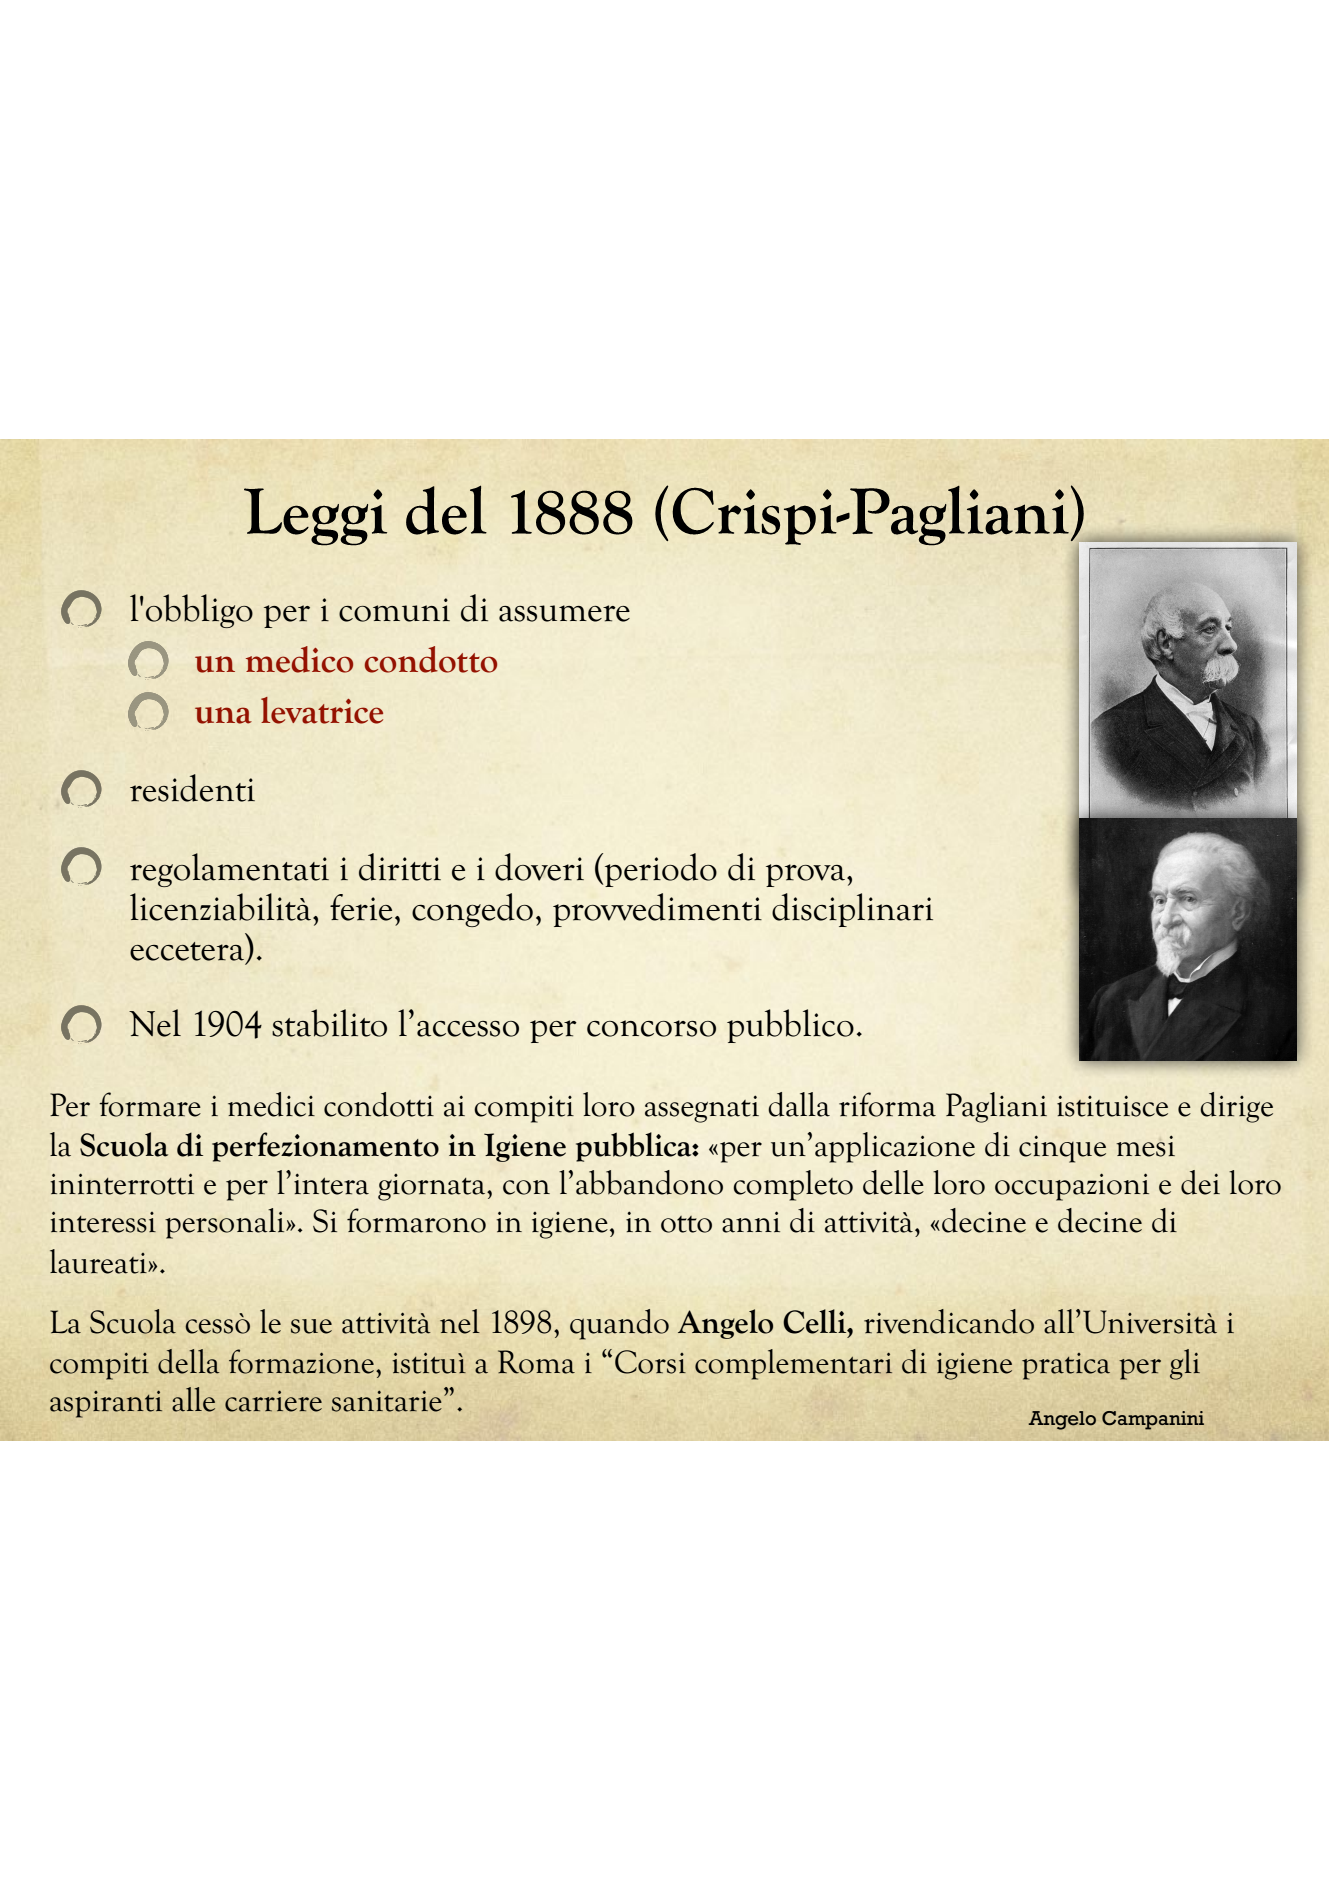
\includegraphics[width=0.8\textwidth]{38/image2.png}
	\end{figure}
	
Con la legge si introduce l'obbligo per i comuni ad avere un medico
condotto e una levatrice. Era dedicato ai residenti ed erano
regolamentati con diritti e doveri. Nel 1904 si accede alle condotte con
concorso pubblico. La scuola di riferimento era la Scuola di
perfezionamento in Igiene pubblica, che cessò rapidamente nel 1898,
quando Celli istituì a Roma ``I Corsi complementari di Igiene pratica
per gli aspiranti alle carriere sanitarie''.

Servì questa riforma? Si poté rilevare, infatti, che tra il 1882 e il
1901,

\begin{itemize}
\item
  la popolazione era aumentata;
\item
  la mortalità generale era diminuita dal 29\% al 20\% ogni 1000
  abitanti;
\item
  la speranza di vita alla nascita era aumentata da 34 a 43 anni;
\item
  l'analfabetismo era diminuito da 62\% a al 48\% ogni 1000 abitanti.
\end{itemize}

Il mestiere del medico condotto di dine Ottocento tuttavia rimaneva un
lavoro duro e poco retribuito.

Qual era la tecnologia dei medici condotti? Se pensiamo all'epoca, la
dotazione dei condotti era straordinariamente avanzata. Era un piccolo
laboratorio di chimica e di tecnologie per l'analisi del paziente.

\begin{figure}[!ht]
\centering
	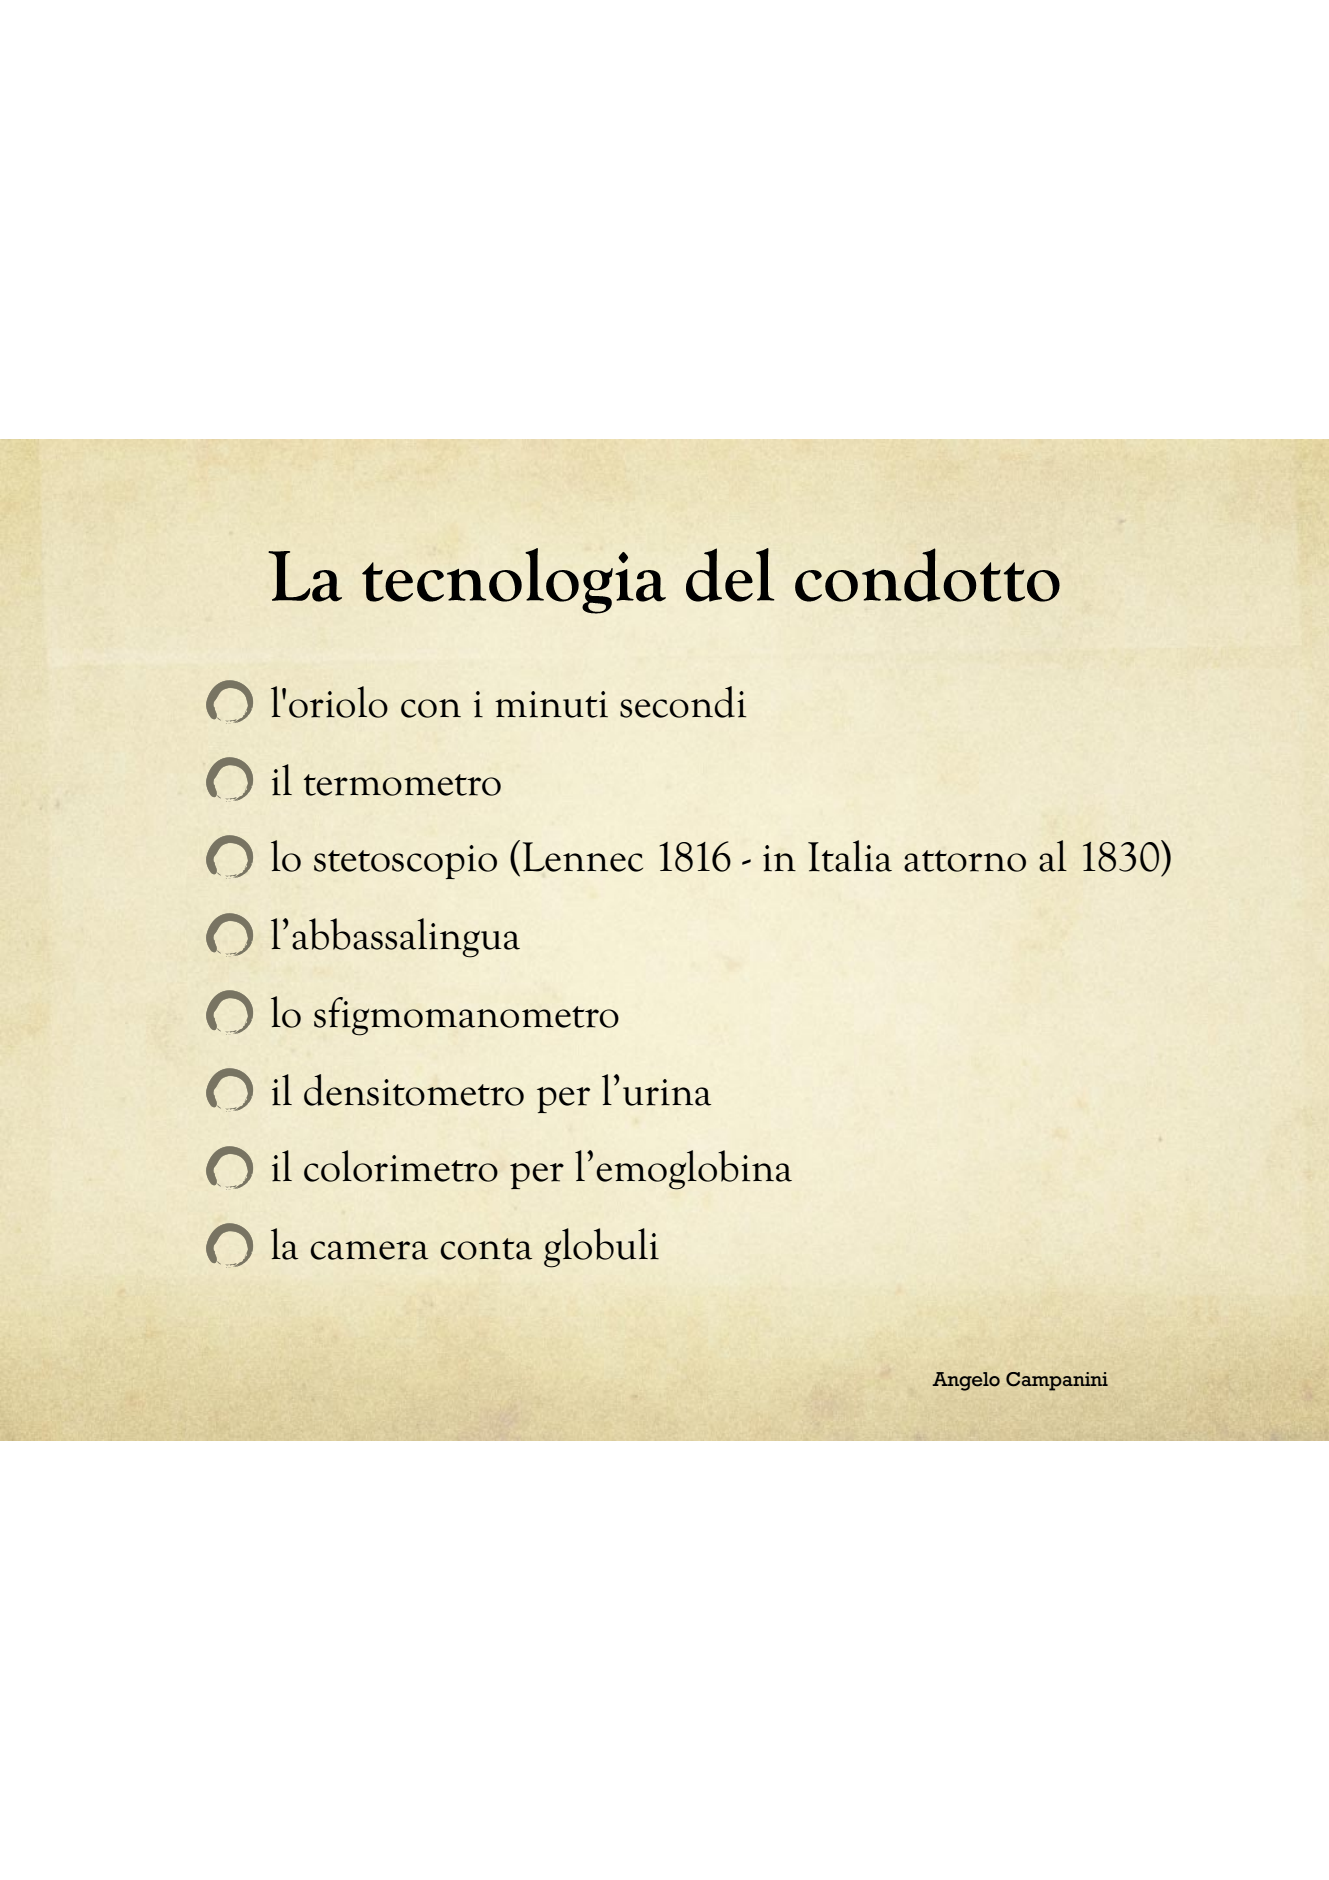
\includegraphics[width=0.8\textwidth]{38/image3.png}
	\end{figure}
	
Dopo la Seconda guerra mondiale, il medico condotto rimane come figura
istituzionale fino alla riforma sanitaria del 1978 che ne ha sancito la
scomparsa giuridica e istituzionale ma ha fortemente improntato
l'immagine, la storia e la pratica della medicina generale italiana.

Nel 1923 viene abolita la condotta piena, perché si erano resi conto che
nessuno voleva farlo a queste condizioni, appena potevano scappavano in
ospedale.

\subsection{Il medico di famiglia}

Compare la figura del medico di Famiglia, differente rispetto al medico
condotto, poiché lavorava in città e seguiva delle famiglie abbienti.
Operava quasi esclusivamente a domicilio o qualche volta faceva consulti
ambulatoriali riservati alla povera gente nel suo studio. Aveva una
visione privilegiata di quello che era il quadro micro-sociale della
famiglia e dell'ambiente, in cui viveva.

Nel corso del Novecento:
\begin{itemize}
\item Aumenta il benessere
\item Il termine ``Medico di famiglia'' si attribuisce ad un medico umano,
confidente, orientato al nucleo familiare, in prima fila per la
battaglia alle sofferenze del vivere quotidiano e senza alcun
riferimento alla salute pubblica. È davvero il medico personale del
paziente e della famiglia.
\end{itemize}

\subsection{Il medico della mutua}

Paradossalmente se non eri povero, non avevi diritto ad avere la
condotta. Per esempio il contadino che lavorava e guadagnava un minimo,
non aveva diritto ad accedere a questo servizio; allo stesso modo
l'operaio.

La Germania vince la guerra Franco-Prussiana contro la Francia e il
principe Otto Bismark viene nominato cancelliere. Bismark convinto che
l'industrializzazione del paese non si potesse realizzare senza misure
di protezione dei lavoratori, introdusse
\begin{itemize}
\item nel 1883 l'assicurazione contro le malattie
\item nel 1884 l'assicurazione contro gli infortuni
\item nel 1889 l'assicurazione contro l'invalidità e la vecchiaia, la
pensione.
\end{itemize}

Perché lo stato si possa sviluppare sul piano economico, lo stato ha
bisogno dei lavoratori e questi hanno bisogno di garanzie. Prese il nome
di ``Sistema Bismarkiano''.

Questo sistema si scontrerà con quello inglese, in cui vigeva ancora la
legge sulla povertà (Poor Law), che prevedeva l'esclusione della chiesa
cattolica da tutte le opere di carità a favore dei poveri e delle
persone in condizioni di bisogno. Quindi il sistema di Bismark fu in
parte imitato dal National Health Insurance nel 1911, che trasforma la
legge sulla povertà del 1837. Il the National Health Insurance riuscì a
modificare la lunga serie di difficoltà dei medici di medicina generale
nei loro rapporti con le autorità laiche locali, assai differenti nella
impostazione dei rapporti professionali, frequentemente basati sulla
gara fra medici a chi offriva il minor prezzo, per assicurare
l'assistenza ad un certo numero di persone.

\begin{figure}[!ht]
\centering
	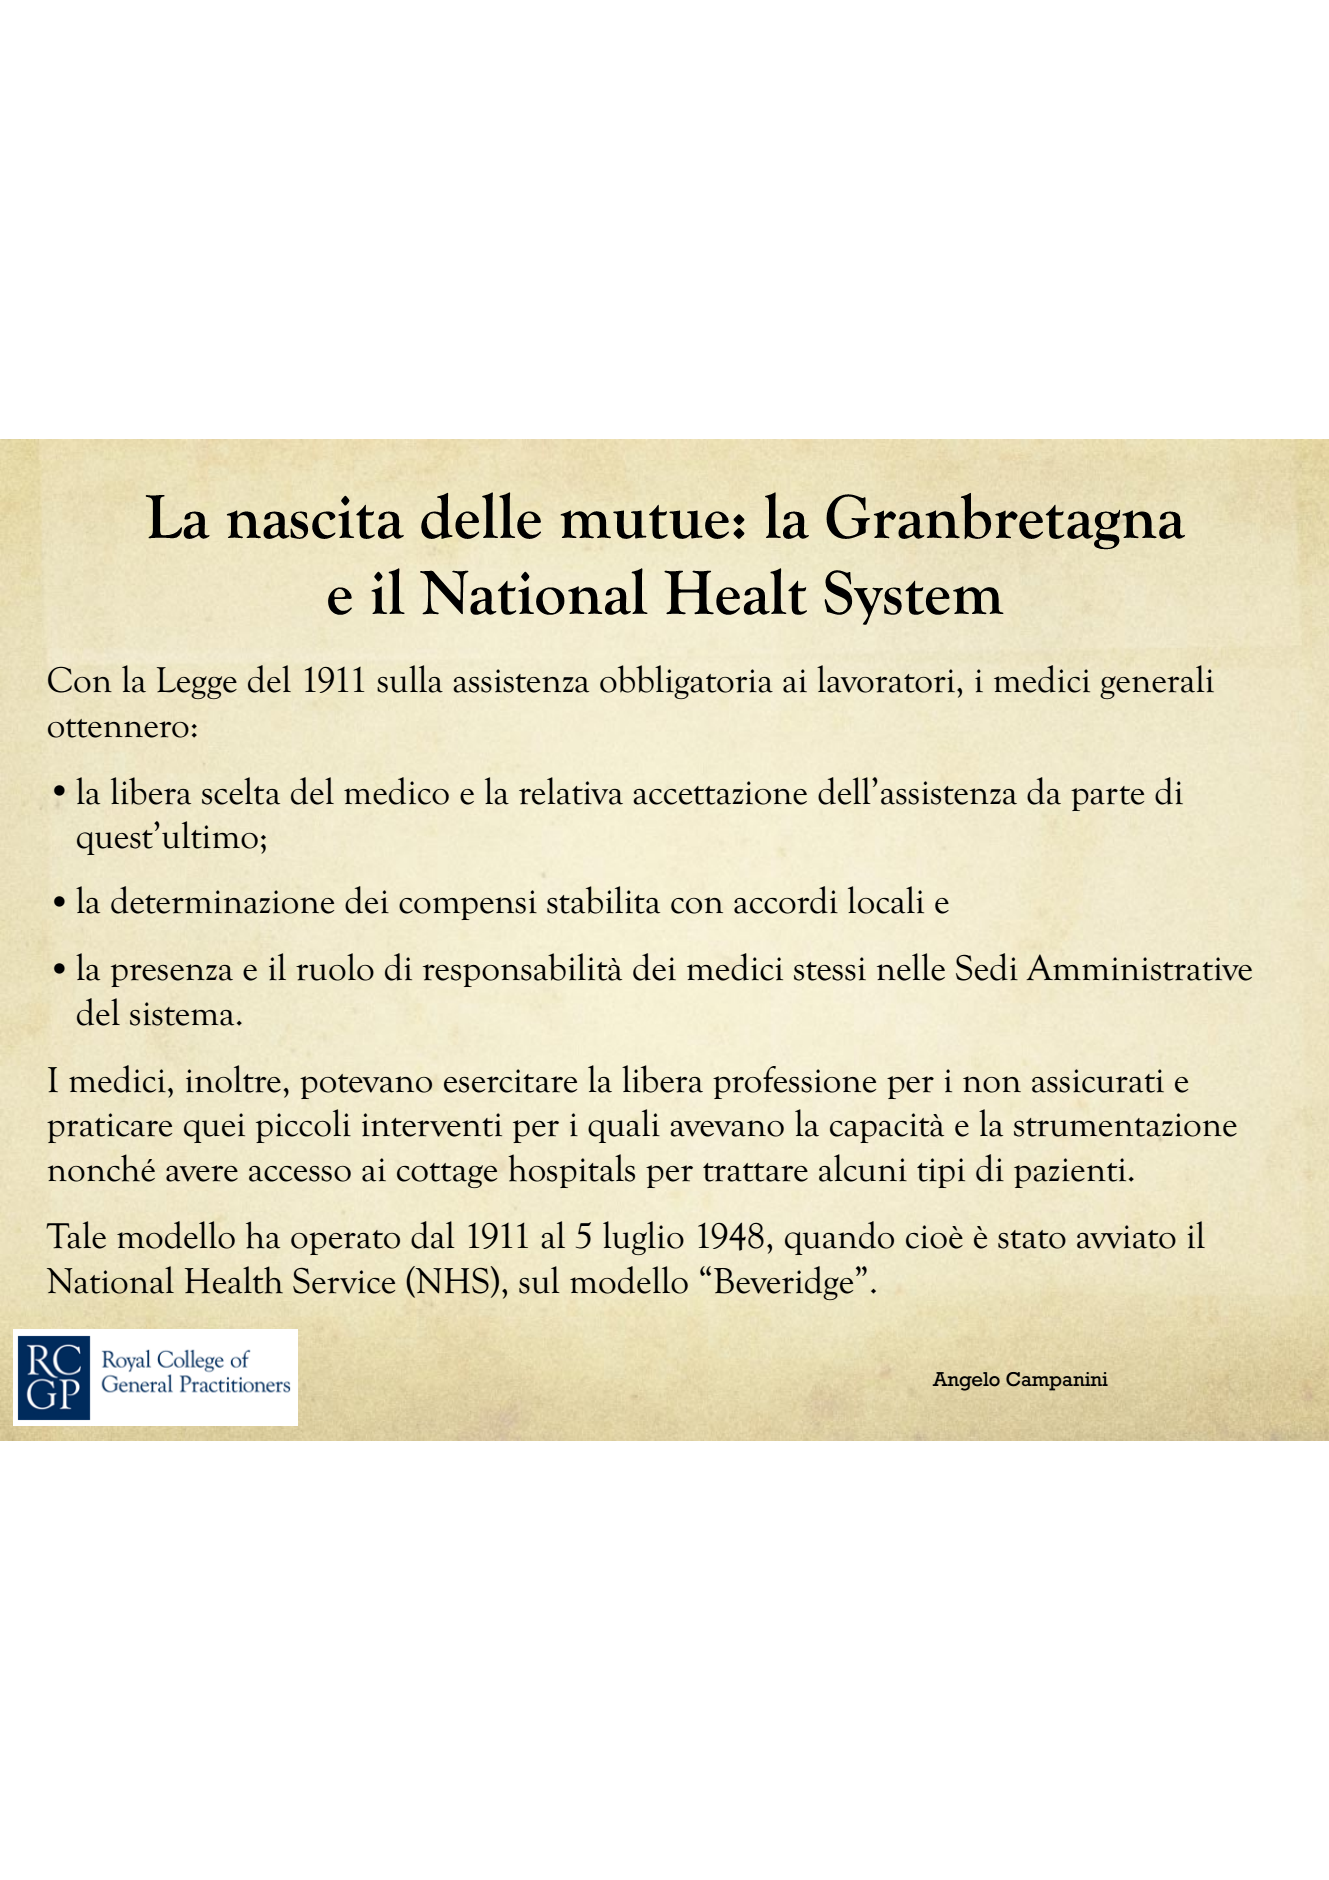
\includegraphics[width=0.8\textwidth]{38/image4.png}
	\end{figure}
	
In seguito la Gran Bretagna cambia orientamento, verso il modello di
Beveridge, esteso a tutti, pagato dalle tasse di tutti i cittadini
presenti nella nazione. Questo è il modello, che ha ispirato poi tutti i
servizi sanitari su base capitaria nazionale, come il nostro del 1978.
\\\\
In Italia cosa succede?

Le prime a nascere sono delle casse private, fatte dagli artigiani e dai
contadini. Avevano il significato di mutuo soccorso: non posso pagarmi
la condotta, verso una piccola quota all'associazione, che pagherà la
condotta per me.

Più avanti, durante il periodo fascista, nel 1934 vengono inserite le
federazioni delle casse mutue dei lavoratori. Nel 1943 vengono unificate
tutte le casse malattia nell'inam, istituto nazionale delle
assicurazioni contro le malattie. Nello stesso periodo nascono l'
``Istituto nazionale fascista per l'assicurazione contro le malattie'' e
l' ``istituto nazionale fascista per la prevenzione sui luoghi di
lavoro'', che rappresentano i nostri moderni l'Inail e l'Inps, istituto
nazionale per la previdenza sociale.
\\\\
Nasce il medico della mutua, che si diffonde soprattutto in città.
Tuttavia, anche alla fine della guerra, la situazione del medico
condotto rimaneva sempre la stessa. Per questo motivo molti condotti,
per arrotondare un po' lo stipendio, si accordarono con le mutue. Le
mutue cominciano a stipendiare i condotti per curare parte dei membri.
In questo modo i condotti possono guadagnare qualcosa in più e
progressivamente il condotto si trasforma anche un po' in medico della
mutua.
\\\\
Quindi quello che si viene a creare è uno scenario di questo tipo:

\begin{itemize}
\item
  Medico Ospedaliero
\item
  Medico di Famiglia
\item
  Medico Condotto
\item
  Medico della Mutua
\end{itemize}

Questi termini, che ora sono diventati sinonimi, hanno rappresentato per
molto tempo realtà diverse. Si comincia a spaccare la conoscenza medica
in due realtà. Nella realtà ospedaliera e universitaria si custodisce il
sapere, la scienza, in continuo aggiornamento; nell'attività quotidiana,
portata avanti dal medico della mutua, c'è la pratica. Pratica che non
apporta aggiornamenti ed è legata al guadagno. Qui comincia a crearsi lo
stereotipo del medico di medicina generale, che fa soldi, senza sapere,
facendo solo ricette. Questo concetto purtroppo si è radicato in modo
molto preponderante nel nostro paese.

\begin{figure}[!ht]
\centering
	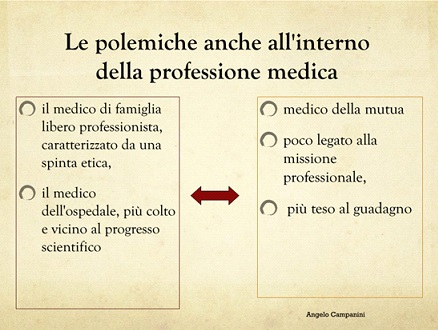
\includegraphics[width=0.8\textwidth]{38/image5.jpg}
	\end{figure}
	
Nel dopo Guerra, il sistema mutualistico si rafforza e si consolida. Si
vengono a creare molti enti, ``pesi massimi'' sono rappresentati da:
\begin{itemize}
\item INAIL, per gli infortuni sul lavoro e le malattie professionali;
\item INAM, per le malattie generiche;
\item INPS, per la tubercolosi, l'invalidità e la vecchiaia.
\end{itemize}

Poi vi erano quelli di minor importanza (``pesi medi''):
\begin{itemize}
\item INADEL, per i dipendenti degli enti locali;
\item ENPDEP, per quelli degli enti di diritto pubblico;
\item ENPALS, per i lavoratori dello spettacolo;
\item ENPAS per quelli statali.
\end{itemize}

Vennero approvate alcune riforme, di cui molto importante fu quella del
1958, dove si istituisce il Ministero della sanità. Oltre ad una
estensione a sempre più numerose categorie, una svolta decisiva alla
mutualità, si ebbe con la legge 841 del 1953, che estendeva l'assistenza
di malattia ai pensionati dello stato e ai loro familiari, e con la
legge 692 del 1955, che estendeva tale beneficio a tutte le altre
categorie di pensionati e ai loro pensionati. Nel 1957 viene introdotta
la cosiddetta Piccola Riforma. Purtroppo per molti anni ben poco cambia
nel panorama sanitario italiano.

Il medico della mutua continua ad essere la figura dominante sul
territorio. Viene immortalato da Sordi in un film di grande successo,
``Il medico della mutua'', dove si mostra proprio il discredito di
questa figura. Il medico è interessato solo all'efficienza, intesa come
la necessità di portare a termine il maggior numero di visite per
ricevere il maggior guadagno. Ma la medicina mutualista resisterà per
anni, immune ai cambiamenti, riforme e anche alla forte satira sociale.
\\\\
Si allarga sempre più lo iato tra la medicina colta, scientifica e la
medicina mutualista sempre più ignorante e ritenuta orientata al
guadagno. Gli ospedali diventano davvero luoghi in cui si va a guarire,
diversamente da un tempo, non più luoghi dove si va a morire o si viene
relegati come in un lazzaretto o in un lebbrosario. Gli ospedali sono i
templi della moderna sanità e della vittoria della salute.

In Europa cominciano a nascere dei college, che riuniscono medici di
medicina generale. Nel mondo anglosassone iniziano a nascere anche i
Dipartimenti di medicina generale. Il peso della medicina generale nella
cultura nord europea è stato per anni completamente diverso rispetto a
quello italiano.

In Italia si è parlato di Medicina in Università soprattutto perché è
scoppiato il boom delle iscrizioni alla facoltà di Medicina. Per fare un
esempio nel 68' all'Università di Parma erano stati registrati 170
iscritti, l'anno successivo 330 iscritti. Questo perché si era data la
possibilità di iscriversi a medicina a tutti, non più solo agli studenti
provenienti dei licei classici e scientifici. Nel 70' gli iscritti
furono 664 e poi 1002, fino a che non si dovette introdurre una
limitazione al numero, in modo da garantire che tutti gli studenti
avrebbero poi trovato un posto di lavoro.
\\\\
Nel 1978 avviene la riforma del Servizio sanitario Nazionale (SSN), che
cancella le mutue. L'Inps e l'Inail rimangono ma con una funzione
diversa. Le altre mutue vengono accorpate e il pagamento di questa mutua
viene versato attraverso le tasse. Il cittadino italiano paga le tasse e
ha diritto all'assistenza sanitaria. Questa riforma fu introdotta a
regime piano piano (Il distretto di Parma si è realizzato quasi
venticinque anni dopo). I distretti nella Regione Emilia Romagna
funzionano da circa vent'anni e la nostra regione è una delle regioni
più virtuose dal punto di vista sanitario.
\\\\
\textbf{LEGGE 833/78} : Ridefinisce il contesto lavorativo del medico del
territorio
\begin{itemize}
\item Assistenza sanitaria universale e allargata a tutti i cittadini
\item Scompaiono dal punto di vista giuridico il medico condotto e il
mutualista
\end{itemize}

\subsection{Il medico di medicina generale}

Nasce il Medico di Medicina Generale, grazie alla legge 833/78. Il MMDG
rappresenta il medico, che aveva una convenzione con le mutue. Questo ha
portato che una moltitudine di medici confluissero nel SSN (circa
30-35.000 medici, che raddoppierà nel giro di 15 anni). Tutti quelli che
avevano una convenzione con le Mutue rientrano nel SSN. In Italia
attualmente si stimano circa 60/68.000 MMDG, di cui quasi la metà già
nel 2020 andrà in pensione.

La prima convenzione con i medici di medicina generale definisce i modi
di reclutamento dei medici, tramite punteggio, e impone i limiti
territoriali di azione del medico, ipotizzandone il collegamento e
l'interazione funzionale con il Distretto Sanitario di base e le
strutture territoriali sociosanitarie di primo livello.

Nascono le società scientifiche nazionali: Società italiana di medicina
generale, l'associazione dei medici di famiglia, l'associazione italiana
di ecografia in medicina generale, e tante altre. Soprattutto con il
tempo si è dimostrato che si può fare ricerca anche in Medicina
Generale, si tratta di ricerca applicata. Cresce l'attenzione a temi
culturali e scientifici che obbligano a precisare e approfondire la
ricerca di uno statuto epistemologico della medicina generale.

\begin{figure}[!ht]
\centering
	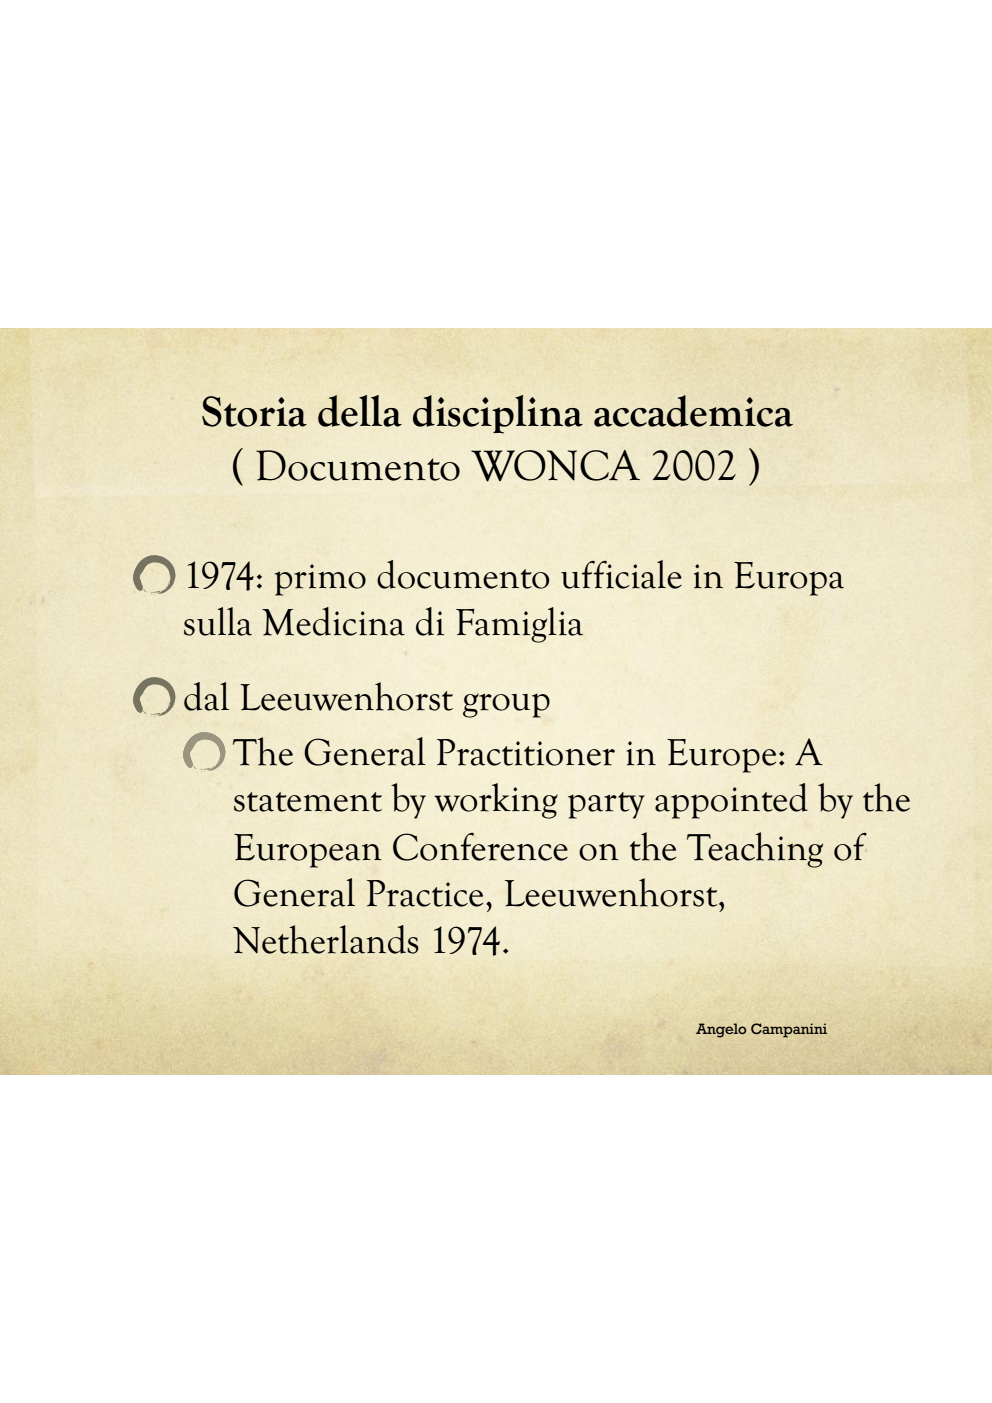
\includegraphics[width=0.8\textwidth]{38/image6.png}
	\end{figure}
	
La medicina generale è una professione olistica, che guarda l'uomo nel
suo complesso, una professione che si basa sulla relazione medico
paziente. Le prime dichiarazioni hanno origine nel 1974 da questo
``Gruppo Leeuwenhorst'', rimasto famoso in Europa.

Questo gruppo redige questa definizione del MMDG:

\begin{figure}[!ht]
\centering
	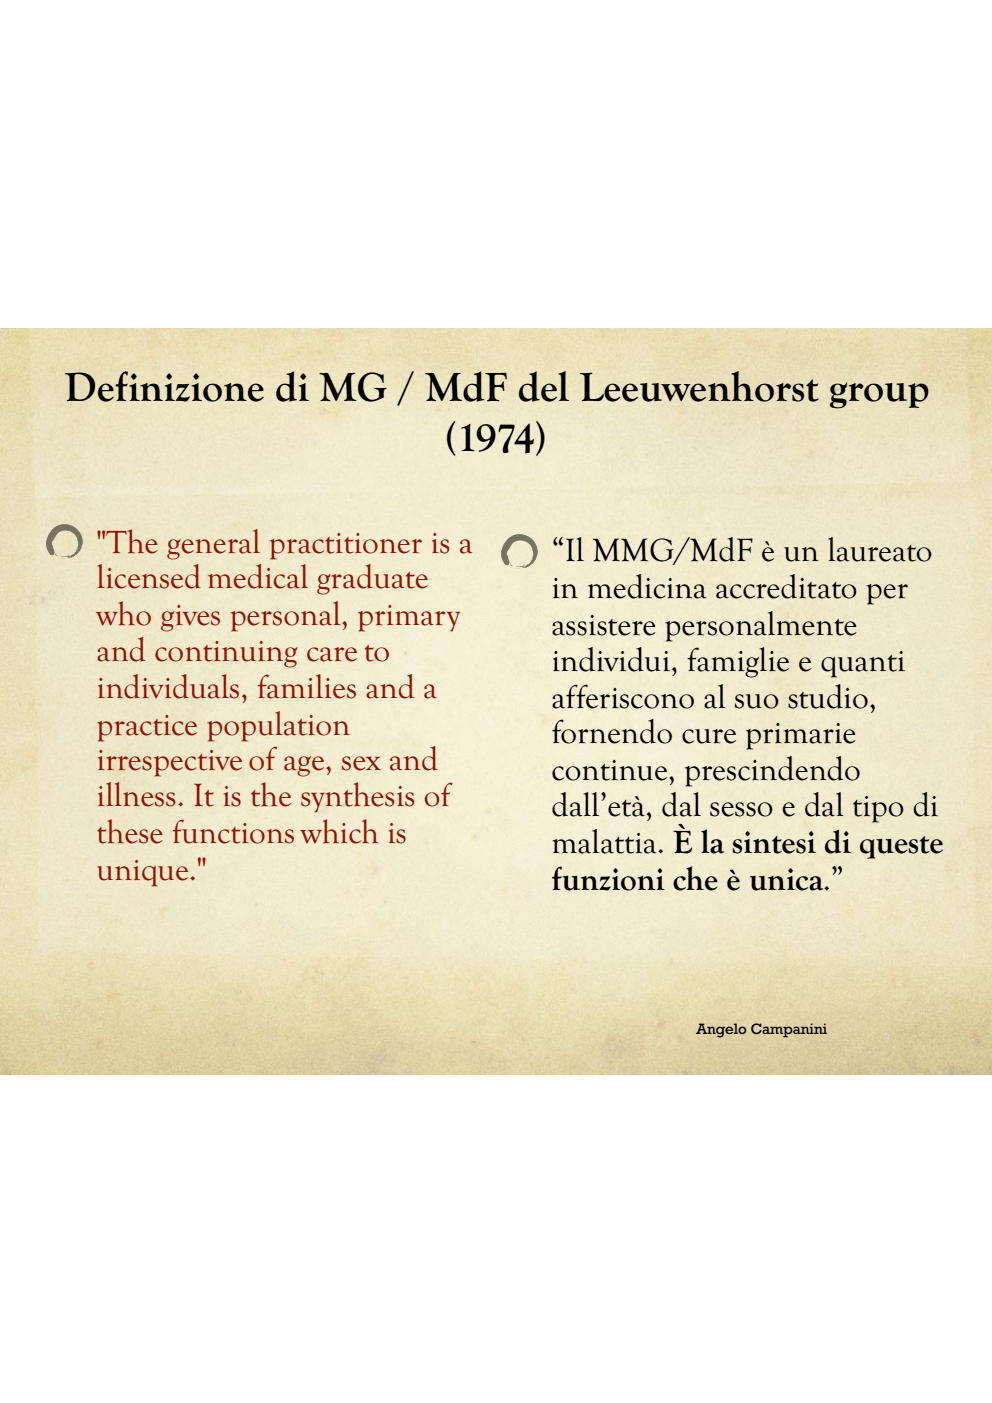
\includegraphics[width=0.8\textwidth]{38/image7.png}
	\end{figure}
	
Più avanti nel 2002, i vari network di questa associazione ``World
Organization of National Colleges and Academies'' (WONCA), che raccoglie
tutti i medici di medicina generale del mondo indipendentemente dai
sistemi politico sanitari all'interno dei quali sono immersi, ha
promulgato una nuova dichiarazione.

La Medicina General è una disciplina accademica e scientifica, con un
proprio contenuto educativo, una metodologia di ricerca, una attività
clinica basata sull'evidenza (Evidence based, Sacket, 1966) ed una
specializzazione clinica rivolta all'assistenza primaria e
nell'assistenza primaria ha degli interessi rivolti all'individuo ma
anche alla collettività nella quale l'individuo è inserito. La ricerca
che si può effettuare è soprattutto quantitativa (es. quante persone
entrano nell'ambulatorio per un determinato motivo).

\begin{figure}[!ht]
\centering
	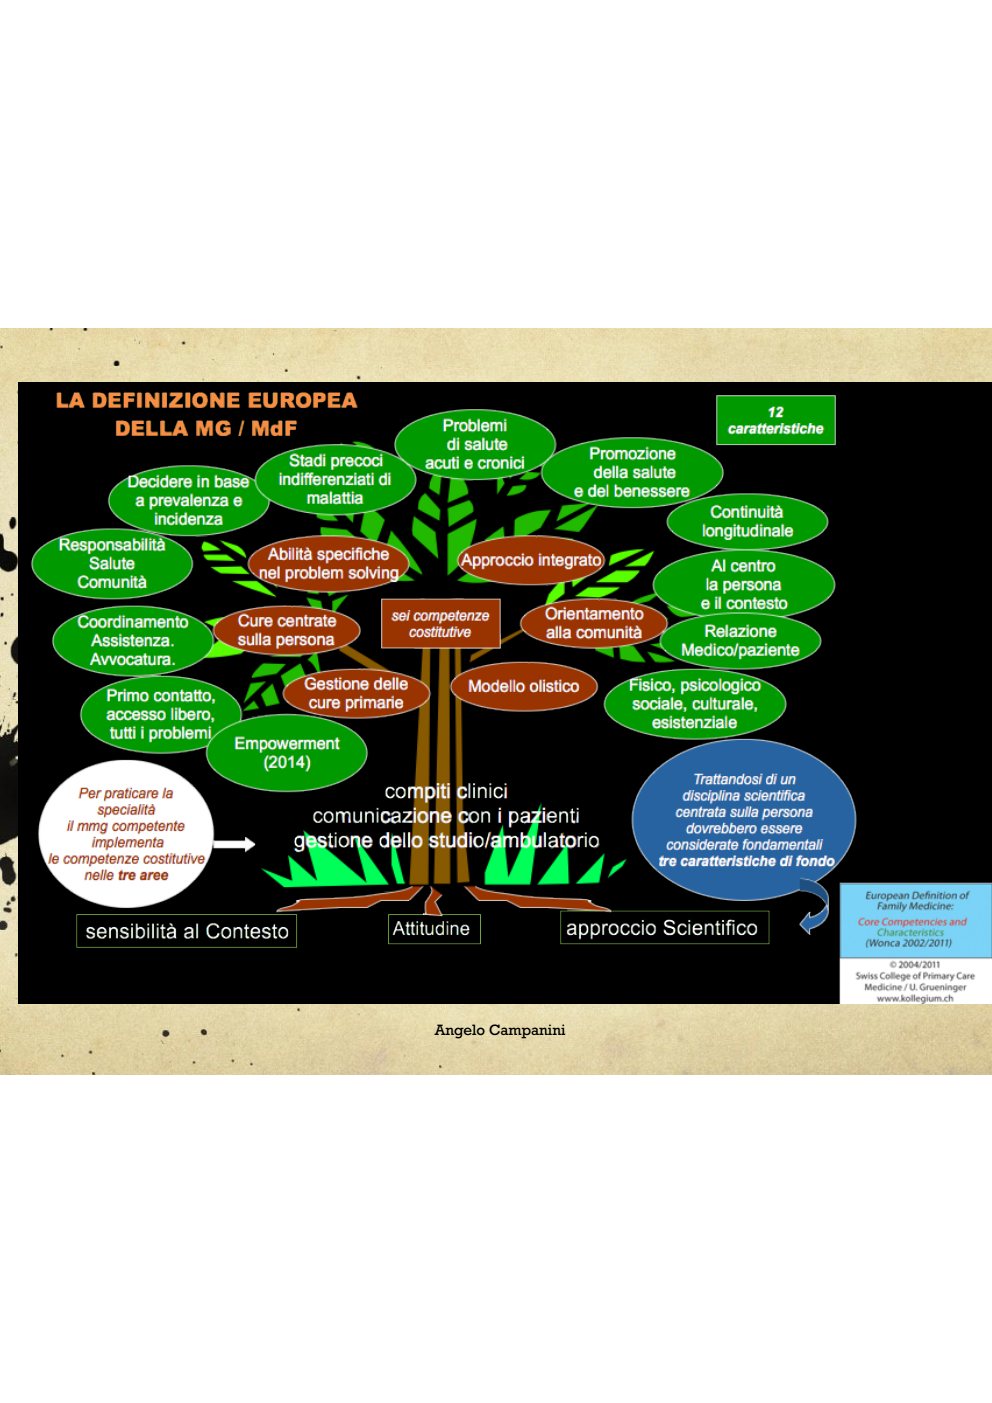
\includegraphics[width=0.8\textwidth]{38/image8.png}
	\end{figure}
	
Questo è l'albero che rappresenta graficamente la Dichiarazione Wonca.
Secondo la definizione, il MMDG dovrebbe essere sensibile al contesto,
nel quale opera; avere una certa attitudine nel fare questo mestiere;
avere un corpo di conoscenze scientifiche tale da consentigli di farlo;
un sistema centrale di competenze che vanno dalla conoscenza dei sistemi
gestionali al fatto che so che la cura è centrata sull'individuo e non
sulla malattia, quindi sarà anche legata a variabili, che non sono
presenti in altri individui; abilità specifiche basate sul Problem
Solving, cioè sulla capacità di risolvere problemi nel momento stesso in
cui si presentano; un approccio integrato, che guarda alla comunità e
segue i criteri del maestro Ippocrate con il modello Olistico. Questo
vuol dire però che ho dodici caratteristiche lavorative imprescindibili.
Il paziente non paga ticket per andare dal MMDG, quindi questo deve
essere anche in grado di coordinare l'assistenza. Al MMDG arrivano le
risposte da tutti gli specialisti e questo deve essere in grado in
ultimo di dare una riunificazione, in modo da capire qual è
effettivamente la soluzione al problema del paziente. Il MMDG è chiamato
in prima linea a rispondere alle problematiche emergenti nei confronti
della collettività (es. SARS). La valutazione che il medico riporta al
paziente è basata sulla prevalenza e incidenza delle malattie, in quel
determinato periodo. Campanini riporta l'esempio della Meningite. Per
esempio il giorno prima ha ricevuto in ambulatorio 17 chiamate di
pazienti, che volevano capire se vaccinarsi o meno per la Meningite e la
sua valutazione è stata basata su un discorso di tipo epidemiologico,
ovviamente sostenuto dagli uffici di Igiene e dall'Agenzia sanitaria
Regionale.
\\\\
DOMANDA: Qual è stata la sua risposta? La risposta è ovviamente graduata
perché siamo calati nel contesto. Se la domanda è relativa ad un bambino
piccolo, bisogna integrare la vaccinazione (sia B che C). Questo perché
è vero che il discorso attuale è legato soprattutto alla situazione
della Toscana, ma non possiamo essere sicuri che fra qualche anno non
tocchi anche la nostra regione. Se la domanda è relativa ad un adulto,
non bisogna alimentare la fobia collettiva. Dopo i 25 anni l'indicazione
alla vaccinazione cala, quindi non vi è la necessità. L'assurdità di
questo fenomeno sta nel fatto che molto spesso il paziente i lamenta
della vaccinazione, come succede per la vaccinazione antinfluenzale, ma
poi vuole sottoporsi ad una vaccinazione più pesante come quella
antimengogoccica. In sostanza riferisco quello che riporta la circolare
della Regione, non esiste motivo attuale di preoccupazione. Nel 2016 è
stato registrato 1 solo caso in Emilia Romagna.
\\\\
Il Medico deve avere come obiettivo personale la promozione della Salute
e del benessere (es. consigliare di smettere di fumare). Il MMDG è
inserito in un contesto di continuità longitudinale. Si seguono dei
pazienti. Al centro c'è la persona, calata nel contesto nel quale vivo.
Agisco su un modello che prende il nome di Bio Psico sociale affronto le
malattie non solo dal punto di vista della semeiotica fisica ma anche
del colloquio. Qualche medico esaspera anche questo concetto e porta
avanti percorsi di psicoterapia. Infine rientra all'interno della
dichiarazione l'Empowerment cioè la capacità di rendere il paziente
corresponsabile della gestione della propria malattia ed è fondamentale
non nel processo patologico acuto ma nel percorso di gestione delle
malattie croniche.

\begin{figure}[!ht]
\centering
	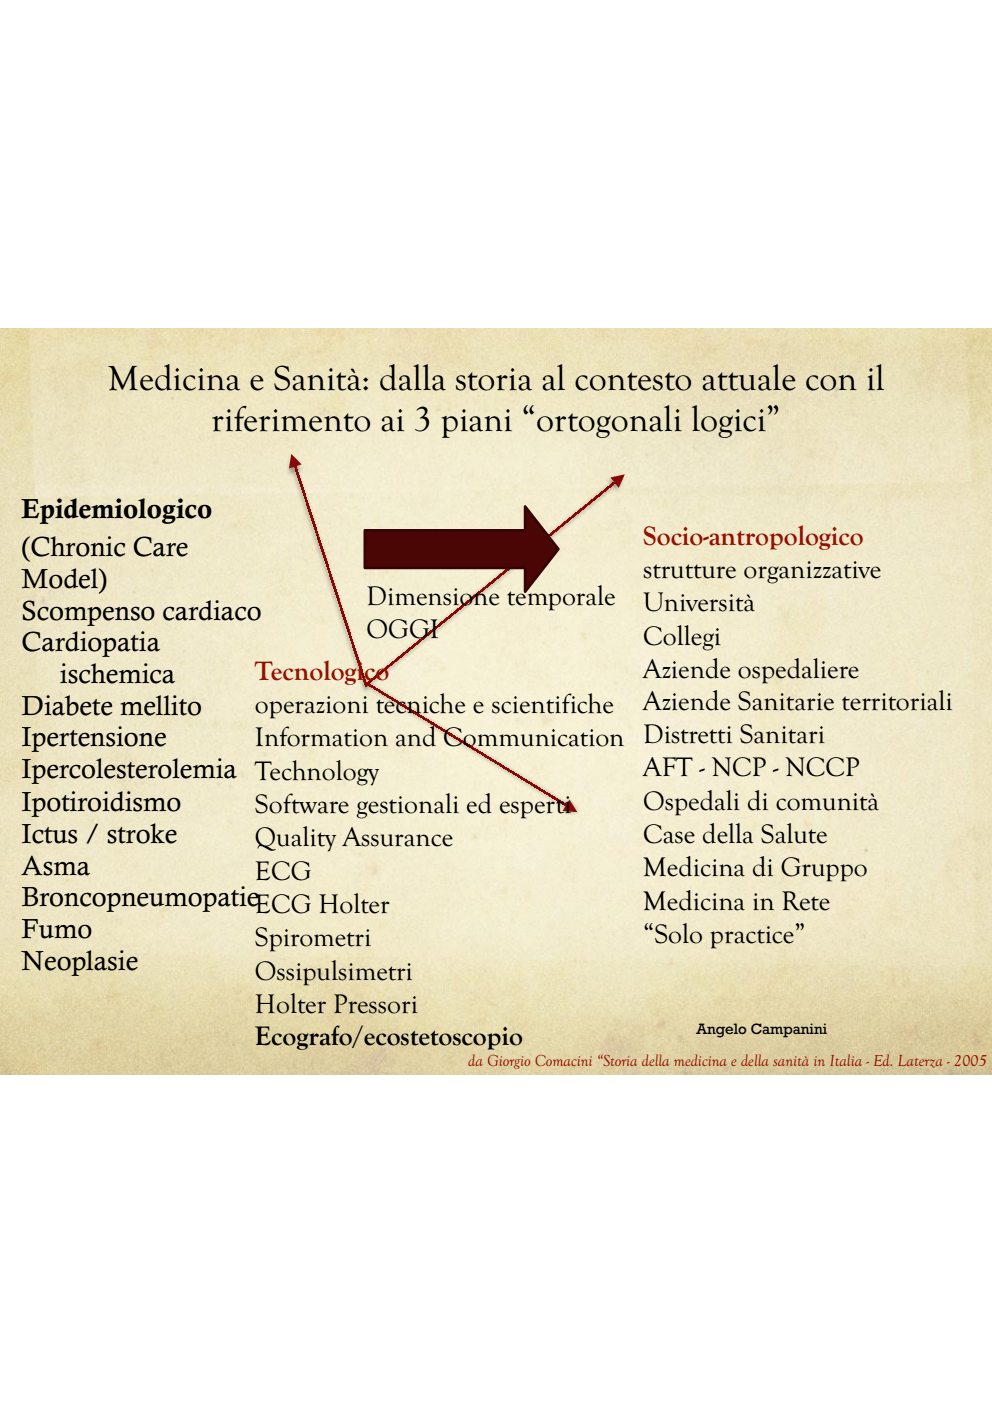
\includegraphics[width=0.8\textwidth]{38/image9.png}
	\end{figure}
	
Se riprendiamo quegli assi ortogonali, che abbiamo già visto nella
lezione precedente, ci accorgeremo che il contesto è cambiato
radicalmente. Il modello epidemiologico pone l'attenzione sulle malattie
croniche e per permettere questo, necessita di un sistema organizzato,
estremamente orientato al territorio. Per esempio nella realtà di
Fidenza fino al 2005 nell'ospedale di zona erano presenti 464 letti, a
seguito della ristrutturazione sono scesi a 119. I pazienti che per
motivi logistici non possono più essere ricoverati, vengono curati a
casa e ricadono nell'ambito di competente del medico di medicina
generale. Inoltre è cambiata la tecnologia. Un Ecg Holter costa molto
3500 euro ma il discorso di molti medici di medicina generale è che,
attrezzandosi, si ottiene un risparmio molto maggiore. Si riescono ad
offrire dei servizi molto più rapidi, efficaci e efficienti sul
territorio, senza necessità di avere delle interfacce. Chiaramente se
l'accertamento diagnostico necessita di un maggior lavoro, si procederà
verso un esame diagnostico di secondo livello. Il MMDG ha bisogno di una
preparazione che è bassa ma ampia perché vede tutto, tutte le
problematiche dalla testa ai piedi, mentre lo specialista ha una
preparazione specializzata in un solo ambito.

\begin{figure}[!ht]
\centering
	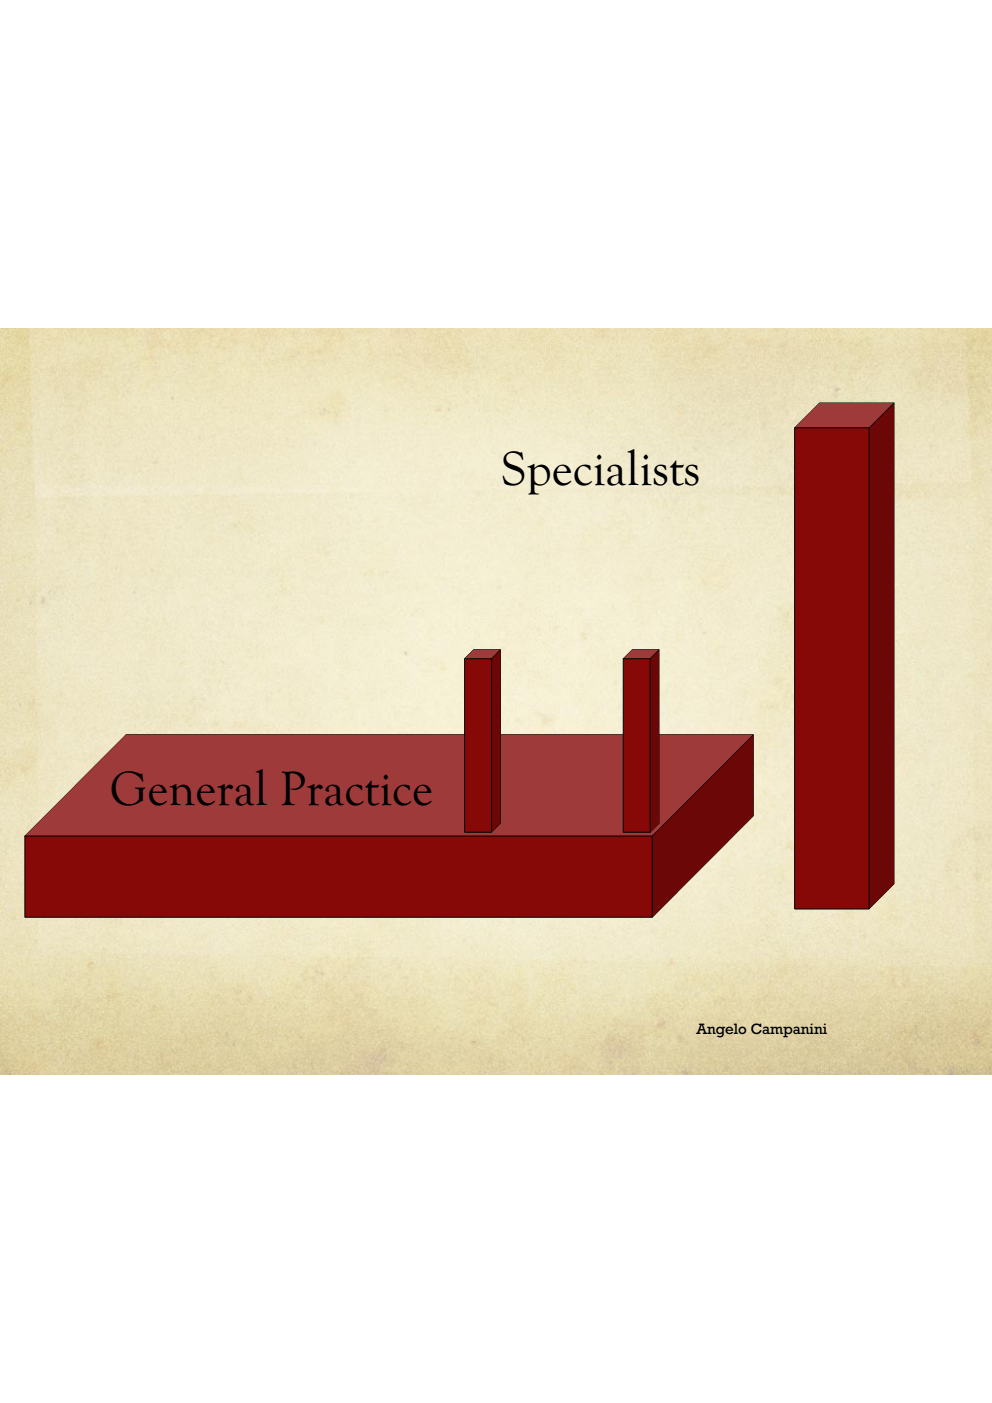
\includegraphics[width=0.8\textwidth]{38/image10.png}
	\end{figure}
	
Nella seconda parte della lezione viene affrontato il discorso più
specifico dell'utilizzo delle tecnologie nella pratica di medicina
generale. Questa esigenza nasce dalla necessità di dare risposte
immediate ai pazienti, che tenga conto di quello che è il contesto
economico e tecnologico della realtà sanitaria italiana.
\\\\
Nella legge 552/92, che ha riformato le unità sanitarie locali
trasformandole in aziende sanitarie con una visione industriale del
prodotto, si sono affermati anche i concetti di Efficacia e Efficienza.
Insita nella legge vi era anche l'idea che in un futuro si sarebbe
tornati alle mutue, ora rappresentate dalle assicurazioni. In un
contesto di questo tipo, alcuni medici di medicina generale hanno
sentito la necessità di raggrupparsi per dare delle riposte multiple,
meglio strutturate. Nacquero così le cooperative, qui in Emilia Romagna,
a Reggio e poi si diffusero in un tutto il resto del paese. In un
secondo momento, nacque sempre nella nostra regione anche la Medicina in
Rete, che si fonda sullo stesso principio delle cooperative ma con un
costo minore dal punto di vista giuridico-amministrativo, non più
fondata su un presupposto legale ma sulla ``Communication and
information tecnology'' in grado di mettere in collegamento più medici
fra di loro attraverso un network informatico. La Medicina in Rete è una
forma organizzativa di medici, che non lavorano nello stesso studio ma
hanno una base comune informatica. È stata successivamente introdotta
anche nell'Accordo collettivo nazionale. L'evoluzione successiva fu il
passaggio alla Medicina di gruppo.
\\\\
Arrivati a questo punto si aveva il panorama dei medici di base era
molto vario: alcuni raggruppati in cooperative, altri in gruppi, pochi
in rete e molti medici operavano ancora singolarmente nel proprio
ambulatorio. Questo è stato lo scenario fino a quando lo stato non ha
deciso di istituire i ``Nuclei di cura primarie'', nuclei di lavoro dei
medici di base, che nell'insieme rispondono ad un distretto. Per Esempio
il nucleo di cure primarie di Fidenza è di 17 medici di base facenti
capo al distretto di Fidenza. Il Medico non perde la propria singolarità
ma si trova a doversi relazionare all'interno di un gruppo, costituito
dal distretto e all'interno di quello si trova a rispondere delle
proprie spese, a precisi parametri prescrittivi, ecc.
\\\\
Siamo forse l'unica Regione che conosce le note AIFA. Le note AIFA sono
quelle che limitano la prescrizione di alcuni farmaci a specifiche
situazioni. Le violazioni delle note AIFA, che sono inserite nella legge
di stabilità del Governo, vengono punite nel penale. Si configura come
un procurato danno erariale. Ci sono delle Regioni che hanno imposto ai
medici di patteggiare il ritorno di corrispettivo economico per farmaci
prescritti impropriamente e per le violazioni delle note AIFA per decine
di migliaia di euro. In Germania in questi casi avviene la sospensione.
\\\\
Successivamente, la regione Emilia Romagna ha proseguito in questo
percorso, facendo un ulteriore passo. Propone una struttura
territoriale, individuabile, differente dall'ospedale ma che possa
rappresentare un centro di riferimento sanitario, la ``casa della
salute'', all'interno della quale vengono raggruppati i medici di
medicina generale, i pediatri, i veterinari, l'igiene pubblica, lo
psichiatra, ecc.

Questo discorso era per spiegare qual è la struttura organizzativa
all'interno del quale i Medici di medicina generale sono immersi, e qual
è stata l'evoluzione che l'ha portata ad essere configurata così.
\\\\
Nella nostra realtà sanitaria ci sono due logiche prevalenti, che
pongono la base della medicina generale e della medicina
ospedaliero-universitaria. Lo specialista ospedaliero e il mondo
universitario si confrontano con il problema del paziente con quella che
viene definita, dal punto di vista epistemologico, la puntualizzazione
del paziente. Mi interessa la diagnosi e la cura immediata in acuto. La
proiezione del MMDG invece dura nel tempo, usa il tempo e tollera
l'incertezza nel tempo; non si arriva quasi mai ad una diagnosi
immediata. Se noi rappresentiamo graficamente queste due logiche
differenti avremo che la medicina specialistica può essere equiparata ad
un punto con bordi ben definiti, mentre la medicina generale ad una
nuvola, un concetto molto meno definito e definibile. Questo ha
rappresentato in passato un problema di appetibilità della professione
del MMDG. Spesso gli studenti si iscrivevano alla scuola di
specializzazione in medicina generale come scelta di esclusone, non
essendo riusciti a entrare nella specializzazione desiderata. Ora invece
è in aumento il numero di iscritti che sceglie questa strada per
vocazione. Il paradigma dell'ospedale è rappresentato dal paradigma
dello spazio, quello per cui il paziente ha una struttura riconoscibile
in cui recarsi per ottenere una diagnosi. L'ospedale e lo specialista
ospedaliero porta avanti il privilegio della diagnosi, che si
contrappone al privilegio della prognosi, di cui si fa portavoce la
medicina generale.
\\\\
Ora, compresa l'organizzazione, la paura di molti medici di base fu
quella che nel futuro la loro professione potesse scomparire o potesse
essere sostituita da altre figure sanitarie, i cosiddetti medici di
secondo livello. Queste figure esistono fin dall'antichità, le avevamo
viste anche nel passato con i Cerusici, ecc. Quindi si è cominciato a
pensare che utilizzando competenze ulteriori, si potesse migliorare la
professione ed evitare anche rischi futuri. A questo proposito Campanini
riporta un articolo da lui pubblicato su ``Gastroenterology made easy''
dal titolo ``L'Ecografo nello studio del MMDG: è lo stetoscopio del
terzo millenio?'', per spiegare come l'innovazione e la strumentazione
possano portare un grande contributo alla pratica quotidiana del medico
di base.
\\\\
Un tempo la struttura organizzativa era molto semplice: il paziente si
recava dal medico, questo lo visitava e poteva o scegliere di mandarlo
da uno specialista per valutare un'ipotesi diagnostica o mandarlo in
ospedale per un ricovero. Alla fine tutto ritorna al medico di base, con
una chiara terapia. Ora la situazione è un po' più complessa perché si
sono inseriti nel panorama nuovi servizi per la cura, il trattamento e
la diagnostica dei pazienti. Per esempio ho l'ospedale per acuti, ho una
serie di strutture più specializzate, il medico di medicina generale, le
infermiere territoriali, strutture per specifiche malattie, specialisti
privati, ambulatori per i codici bianchi, infermiere professionali non
inserite nel territorio ma che lavorano sempre privatamente nel
territorio, le assistenze domiciliari integrate, i servizi sociali, ho
gli ospizi, ecc, In sostanza ho una complessità estremamente articolata.
Se noi con l'utilizzo della tecnologia, riusciamo a destinare meglio le
risorse e a essere più appropriati nella diagnosi, rendiamo anche più
accessibili i servizi di secondo livello. La scrematura non può essere
fatta là ma deve essere fatta sul territorio.
\\\\
Quindi la tecnologia mi permette di essere più efficace e se divento
efficace nella diagnosi, lo sono chiaramente, anche dal punto di vista
della cura. Il medico deve affidarsi a qualcosa che lo possa aiutare, la
strumentazione, il modello tecnologico. In più dobbiamo anche pensare a
tutte le possibilità di cui disponiamo con le moderne tecnologie. Un
medico solo con un Ipad e una sonda ecografica può già ottenere delle
prime immagini, in modo da indirizzare la diagnosi. Ed è stato anche
dimostrato che questo modello apporta dei vantaggi. È stata fatto fare
uno studio agli allievi della scuola italiana di ecografia in medicina
generale, durante il quale si sono valutati le tempistiche medie per
arrivare alla diagnosi di pazienti con dolore addominale. Negli
ambulatori in cui era presente l'ecografo, il medico in 2,3 giorni aveva
chiuso la diagnosi, mentre negli altri casi ci hanno messo 41,8 giorni
di media per arrivare ad una diagnosi. Sono dati che parlano da soli.
Chiaramente questo tipo di tecnologia va studiata per poter essere
sfruttata.

Nell'ultima parte della lezione, Campanini riporta una serie di esempi,
con cui supporta l'importanza dell'ecografia nella Medicina generale. A
scopo di esempio riporto un solo caso fra quelli riportati a lezioni.

  \textit{Arriva un paziente di 32 anni, in buona salute, si presenta in
  ambulatorio perché ha notato un'ematuria macroscopica episodica da una
  settimana. Non riferisce dolore, non riesce a puntualizzare se si
  tratti di ematuria iniziale, terminale o totale.}

Quali sono le Ipotesi diagnostiche? -- Cistite emorragica? Trauma?
Problematica renale? Dal punto di vista anamnestico posso chiedere al
paziente se ha visto l'urina con il sangue subito all'inizio della
minzione, alla fine o durante tutto l'atto. Questa domanda ha la stessa
funzione del test di Guyon, dei tre bicchieri. Il paziente tuttavia non
era in grado di ricordare.

L'assenza di dolore esclude la possibilità che si tratti di cistite o
colica renale. Il paziente riferisce di giocare a calcio ma non si ha
anamnesi di trauma, che potrebbero aver causato frattura subcapsulare
del rene. Quindi il Medico di base che possiede l'ecografo procede con
l'ecografia. Utilizzando l'ecografo si nota una masserella, a forma di
cavolfiore nella vescica, anche animato da gettoni vascolari, evidenti
al power doppler. Ragionevolmente si orienta la diagnosi verso il
riscontro di una neoplasia maligna, che necessiterà di ulteriori esami
di secondo livello. La diagnosi è stata fatta in 1 ora! Seguirà
chiaramente una visita in Urologia, pet, ecc. Nel giro di una ventina di
giorni, il paziente viene operato, riuscendo anche ad adottare una
soluzione che gli permetta di mantenere la vescica e anche l'uretere.